\chapter{Historie \legoM}

Historie firmy \lego{ }je velmi dlouhá a sahá až do roku 1932~\cite{lego_GroupHistory1930s}. 
Prakticky to samé lze říct o stavebnici \legoM, jejíž počátky se datují k roku 1998~\cite{lego_mindstormsHistory} (období, během něhož se počítač stával běžnou součástí domácnosti).
% * <lucie.karmova@jcmm.cz> 2017-04-27T13:41:25.667Z:
% 
% > mívat běžní lidé doma
% 
% Lidé běžně doma
% 
% ^ <paral.jarek@gmail.com> 2017-04-27T14:57:29.212Z:
%
% Já jsem to myslel ve stylu, že už se počítače dostávají do domácnosti běžných lidí a ne jenom geeků. Myslíš, že je to lepší přepsat na "lidé běžně doma"?
%
% ^ <lucie.karmova@jcmm.cz> 2017-04-27T19:49:25.460Z:
%
% Zatímco "běžní uživatelé" je zažitý výraz, "běžnými lidmi" bych si tak jistá nebyla a zní mi to krapně pejorativně.
% Co třeba i "období, během něhož se počítač stával běžnou součástí domácnosti"?
%
% ^ <paral.jarek@gmail.com> 2017-04-27T20:30:41.364Z.

% TODO: kapitola LEGO TECHNIC

\section{\legoM{ }RCX}

První verze byla označena jako \legoM{ }RCX\footnote{RCX = Robotic Command eXplorers} Intelligent Brick and Robotics Invention System a  obsahovala 8bitový mikrokontrolér Hitachi H8/3292~\cite{hitachi_microcontrolerH8series} s procesorem H8/300 taktovaným na 16~MHz a~s~32~KB~RAM~\cite{legoMindstormsRCX_Manual}.
% * <lucie.karmova@jcmm.cz> 2017-04-27T13:41:42.843Z:
% 
% >  8bitový
% 
% Viz výše
% 
% ^ <paral.jarek@gmail.com> 2017-04-27T20:28:53.154Z.

\begin{figure}[h]
	\centering
	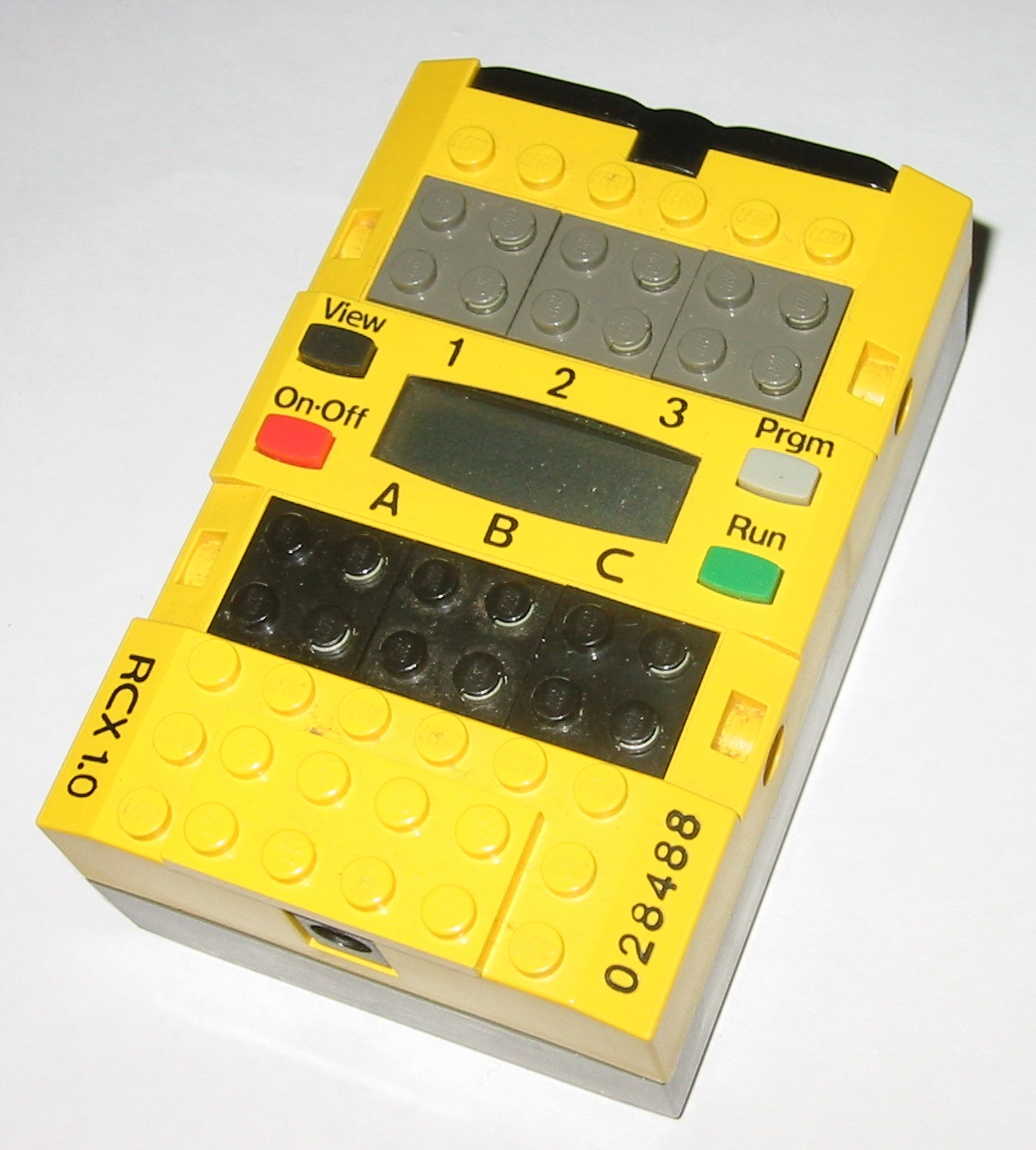
\includegraphics[width=250px]{images/lego-mindstorms-rcx_wikipedia.jpg}
	\caption[\legoM{ }RCX]{\legoM{ }RCX\protect\footnotemark}
	\label{fig:lego-mindstorms-rcx-wikipedia}
\end{figure}

\footnotetext{Zdroj: \url{https://en.wikipedia.org/wiki/Lego_Mindstorms}} 

Oficiálně bylo možné stavebnici programovat ve dvou prostředích. První prostředí ROBOLAB, založené na programu \labview{ }od firmy \NI, bylo pro výukové účely (do škol) a bylo součástí výukového setu. 
Běžní zákazníci (lidé, kteří si kupovali stavebnici domů) měli k dispozici RCX Code, které bylo jednodušší na obsluhu a používání, ale nemělo tak rozsáhlé možnosti programování. 
Zároveň vznikla i vývojová prostředí třetích stran, která umožňovala programování v mnoha běžně používaných jazycích (C++, Java,~\dots).
% * <lucie.karmova@jcmm.cz> 2017-04-27T13:42:39.199Z:
% 
% > vznikly i vývojové prostředí třetích stran, které umožňovali
% 
% 
% vzniklA i vývojovÁ prostředí třetích stran, kterÁ umožňovalA
% 
% ^ <paral.jarek@gmail.com> 2017-04-27T14:15:20.597Z:
%
% Opraveno.
%
% ^ <paral.jarek@gmail.com> 2017-04-27T14:15:25.850Z.

Již v prvním roce prodeje stavebnice vznikla soutěž {\it FIRST} LEGO League (FLL)\footnote{{\it FIRST} = For Inspiration and Recognition of Science and Technology}. 
Cílem soutěže je povzbudit a motivovat k navrhování, stavění a programování vlastních inteligentních systémů~\cite{lego_FLL-about}. 
Jednotlivá kola probíhají po celém světě a lze postoupit až do celosvětového finále. % TODO: FLL - ověřit možnost postupu do celosvětového finále
Účastníci musí být ve věku od 10 do 16 let. 


\section{\legoM{ }NXT}

Následující verzi vydalo \lego{ }v roce 2006~\cite{lego_mindstormsHistory}. 
Byl kompletně změněn způsob připojování jednotlivých modulů. 
Moduly se již nepřipojují pomocí speciálních \lego{ }kostek, ale využívají upravený konektor RJ-12 % TODO: upravený konektor -> méně běžnou variantu konektoru RJ-12
(kolík sloužící pro správné zapojení konektoru je oproti běžné telefonní RJ-12 umístěn mimo střed~\cite{legoMindstorms_rj12-connector}). % -- na pravou stranu z pohledu od kabelu 
% * <lucie.karmova@jcmm.cz> 2017-04-27T13:43:56.040Z:
% 
% > kolík sloužící p
% 
% obě čárky pryč
% 
% ^ <paral.jarek@gmail.com> 2017-04-27T14:18:52.832Z:
%
% Takhle "sloužici"? Proč to tak má být? Nikde jsem k tomu nenašel žádné vysvětlení :-| (všude má obě čárky).
%
% ^ <lucie.karmova@jcmm.cz> 2017-04-27T19:50:47.643Z:
%
% Neee, promiň, je to samozřejmě "kolík". Myslela jsem čárky před "je" a "umístěn".
%
% ^ <paral.jarek@gmail.com> 2017-04-27T20:27:13.643Z:
%
% Opraveno.
%
% ^ <paral.jarek@gmail.com> 2017-04-27T20:27:32.241Z.

\begin{figure}[h]
	\centering
	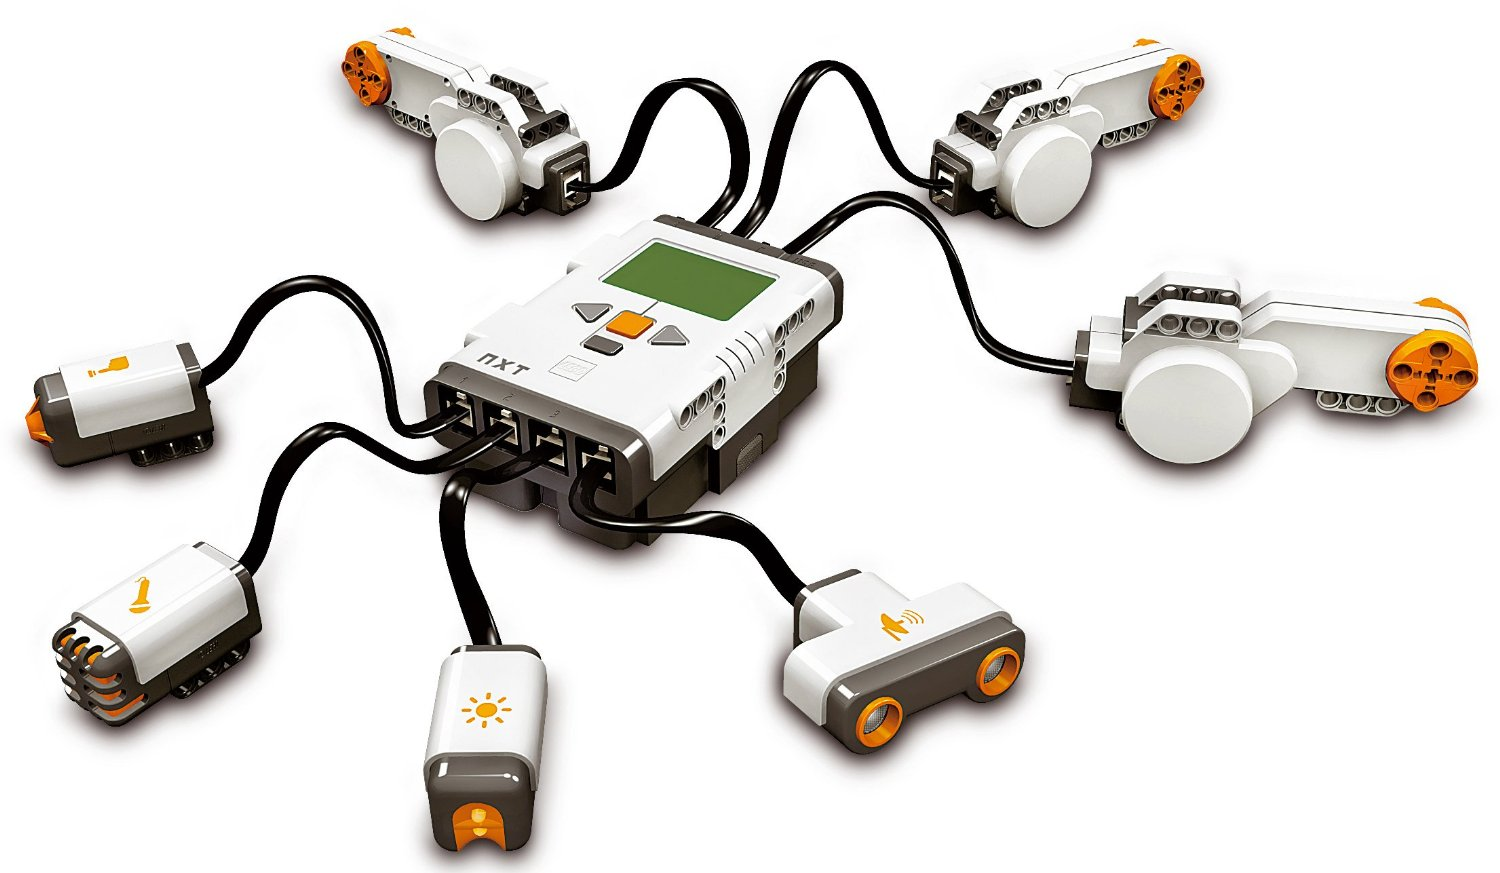
\includegraphics[width=\textwidth]{images/lego-mindstorms-nxt_with-modules.jpg}
	\caption[\legoNXT{ }s komponenty, které lze používat]{\legoNXT{ }s komponenty, které lze používat\protect\footnotemark}
	\label{fig:lego-mindstorms-nxt_with-modules}
\end{figure}

Řídicí kostka (dále jen \brick{}) % TODO: formátování speciálních výrazů
% * <lucie.karmova@jcmm.cz> 2017-04-27T13:44:24.268Z:
% 
% > Řídící
% 
% Řídicí, viz výše
% 
% ^ <paral.jarek@gmail.com> 2017-04-27T14:19:10.131Z:
%
% Opraveno.
%
% ^ <paral.jarek@gmail.com> 2017-04-27T14:20:15.962Z.
se již neprogramuje přes infraport, ale využívá se standardní USB kabel, případně integrovaný Bluetooth~\cite{legoMindstormsNXT_hardware}.

Po hardwarové stránce došlo ke značnému posunu. Původní 8bitový mikrokontrolér byl nahrazen 32bitovým ARM mikrokontrolérem % TODO: mikrokontrolér/mikroprocesor/procesor
% * <lucie.karmova@jcmm.cz> 2017-04-27T13:45:04.060Z:
% 
% > í 8bitový mikrokontrolér byl nahrazen 32-bitovým
% 
% Bez spojovníků
% 
% ^ <paral.jarek@gmail.com> 2017-04-27T14:20:36.984Z:
%
% Dořešit.
%
% ^ <paral.jarek@gmail.com> 2017-04-27T20:28:59.136Z.
AT91SAM7S256 (256~KB~FLASH, 64~KB~RAM, 48~MHz) a k němu byl přidán 8bitový ko-procesor ATmega48 (4~KB~FLASH, 512~Byte~RAM, 8~MHz). 
% * <lucie.karmova@jcmm.cz> 2017-04-27T13:45:24.113Z:
% 
% > 8bitový
% 
% Ale to už si umíš když tak pohlídat, ne?
% 
% ^ <paral.jarek@gmail.com> 2017-04-27T14:21:06.834Z:
%
% JJ
%
% ^ <paral.jarek@gmail.com> 2017-04-27T20:29:03.149Z.
Oba tyto procesory dodávala firma Atmel (nyní již Microchip)~\cite{legoMindstormsNXT_hardware}.

\footnotetext{Zdroj: \url{http://www.itnetwork.cz/java/lego-nxt/seznameni-s-nxj-pro-lego-nxt}} 

\brick{ }lze programovat pomocí vývojového prostředí NXT-G\footnote{NXT-G = NXT Graphic - grafické} (viz obrázek \ref{fig:lego-mindstorms-nxt-g}), které \lego{ }vyvinulo opět ve spolupráci s  \NI{~}\cite{legoMindstormsNXT_NXT-G}. 
Zároveň \NI{ }dodává toolbox do \labview{ },ve kterém lze \brick{ }také programovat. 
% * <lucie.karmova@jcmm.cz> 2017-04-27T13:46:08.604Z:
% 
% > toolbox do \labview{ }ve kterém lze \brick{ }také 
% 
% Před "ve" patří čárka, máš za ní celou větu.
% 
% ^ <paral.jarek@gmail.com> 2017-04-27T14:21:53.179Z:
%
% Opraveno.
%
% ^ <paral.jarek@gmail.com> 2017-04-27T14:21:55.656Z.

\legoNXT{ }má ovšem bohatou nabídku alternativních programovacích prostředí, která lze využít k vytváření kódu pro \brick. 
% * <lucie.karmova@jcmm.cz> 2017-04-27T13:46:34.867Z:
% 
% > které
% 
% KterÁ
% 
% ^ <paral.jarek@gmail.com> 2017-04-27T14:22:12.130Z:
%
% Opraveno.
%
% ^ <paral.jarek@gmail.com> 2017-04-27T14:22:13.600Z.
Některá fungovala již na RCX a byla upravena i pro NXT. 
% * <lucie.karmova@jcmm.cz> 2017-04-27T13:46:56.584Z:
% 
% > Některé fungovali již na RCX a byly upraveny 
% 
% Bavíme se o prostředí, že? Takže fungovalA a bylA upravenA
% 
% ^ <paral.jarek@gmail.com> 2017-04-27T14:25:06.796Z:
%
% Opraveno. Nemá být pak přepsán i "Některé" => "Některá"?
%
% ^ <lucie.karmova@jcmm.cz> 2017-04-27T19:53:40.025Z:
%
% Jo, uteklo mi.
%
% ^ <paral.jarek@gmail.com> 2017-04-27T20:25:00.734Z.
Jako příklad mohu uvést jedno z nejpoužívanějších prostředí BricxCC\footnote{BricxCC = Bricx Command Center} s jazykem NXC\footnote{NCX = Not eXactly C}. 
NCX je vysokoúrovňový open-source jazyk podobný C~\cite{legoWikipediaNXT_NXC}.

\begin{figure}[h]
	\centering
	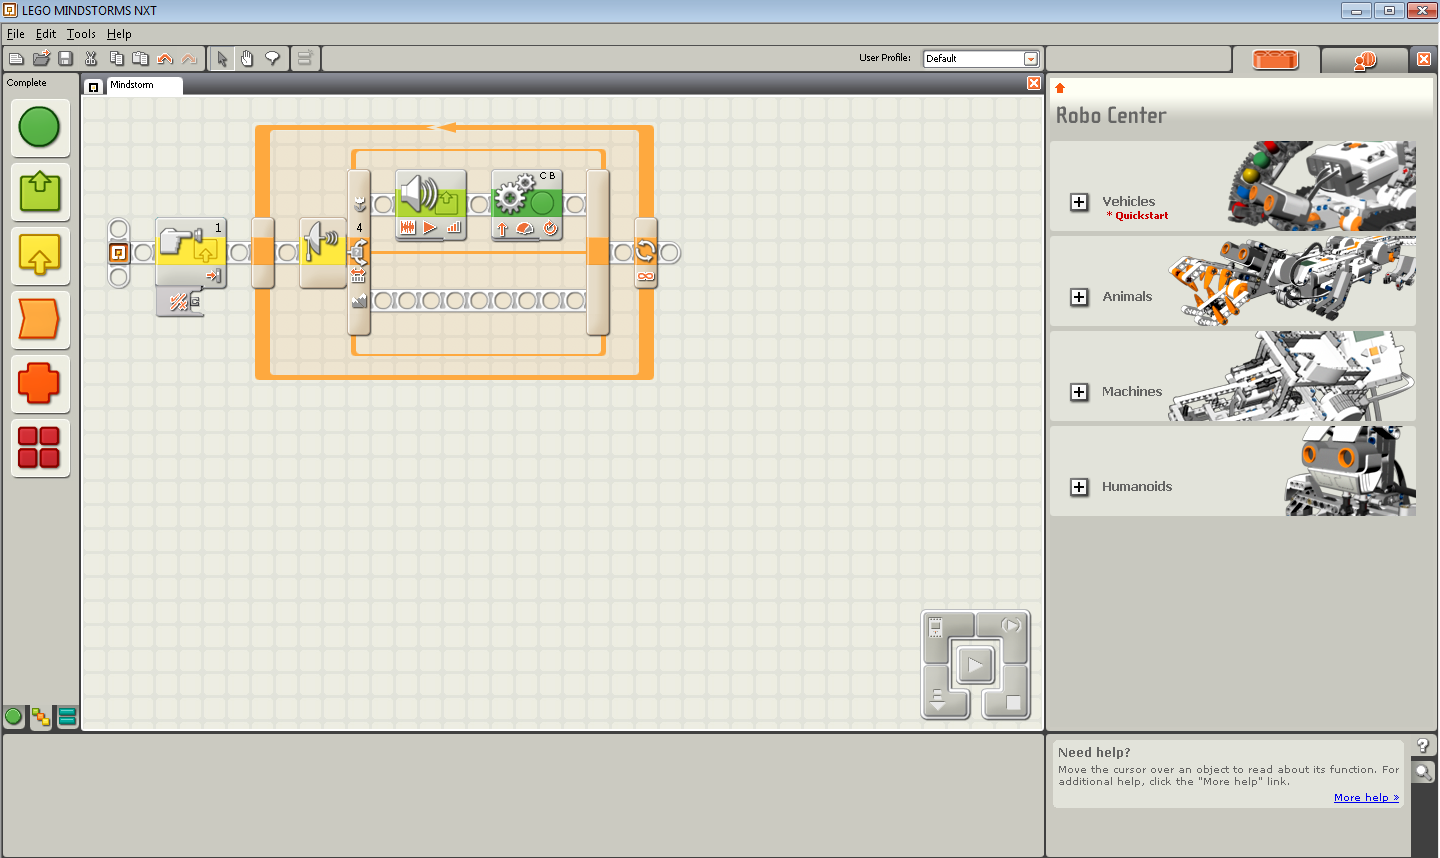
\includegraphics[width=\textwidth]{images/lego-mindstorms-nxt-g.png}
	\caption[\legoNXT{-G}]{\legoNXT{-G}\protect\footnotemark}
	\label{fig:lego-mindstorms-nxt-g}
\end{figure}

\footnotetext{Zdroj: \url{http://lukedainton-robots.blogspot.cz/2012/07/control-systems-shooterbot-nxt-g.html}} 
Existují ale i komerční varianty. 
Například ROBOTC~\cite{legoProgramingPlatform_ROBOTC} je univerzální programovací prostředí a jazyk umožňující programovat větší množství hardwaru (od \legoM{ }RCX, NXT, EV3 až po Arduino nebo PIC). 
Jak již název napovídá, ROBOTC je založen na jazyku C (ANSI-C).
Uživatel ovšem může přecházet mezi grafickou a textovou formou programování, což může být pro začátečníky velmi vhodné.
Také má možnost vybrat si úroveň abstrakce, na jaké bude v textovém módu pracovat.  
% * <lucie.karmova@jcmm.cz> 2017-04-27T13:47:58.216Z:
% 
% >  abstrakce na jaké
% Před "na" patří čárka, je za ní věta.
% 
% ^ <paral.jarek@gmail.com> 2017-04-27T14:26:03.715Z:
%
% Opraveno.
%
% ^ <paral.jarek@gmail.com> 2017-04-27T14:26:04.591Z.
ROBOTC je velmi zajímavé prostředí. Bohužel nikdy nebyla vydána objektová varianta, s kterou by mohlo být programování ještě jednodušší. 
Zároveň se jedná o placený produkt a jednotlivé licence~\cite{legoProgramingPlatform_ROBOTC-price} tvoří přibližně čtvrtinu současné ceny základní sady stavebnice \legoEV{~}\cite{lego_eduxeEshop_CoreSet}, což už není nezanedbatelná částka.

Pro NXT existuje celá řada dalších platforem a jazyků (Javy, C\#, Lua, Ada, Python~\cite{legoMindstormsNXT_Programming}), které lze použít. 
Jelikož je ale tato práce zaměřena na \legoEV{ }, nebudou tyto platformy dále řešeny. 
% * <lucie.karmova@jcmm.cz> 2017-04-27T13:48:42.480Z:
% 
% > nebudou
% Před "nebudou" patří čárka, je je za ní věta.
% 
% ^ <paral.jarek@gmail.com> 2017-04-27T14:26:51.802Z:
%
% Opraveno.
%
% ^ <paral.jarek@gmail.com> 2017-04-27T14:26:53.014Z.


\section{\legoM{ }EV3}

Aktuálně nejnovější verzí stavebnice \legoM{ }je verze EV3, která byla vydána v roce 2013~\cite{lego_mindstormsHistory}. 
Proběhlo u ní mnoho inovací a změn, i tak ale byla zachována velmi dobrá kompatibilita s verzí NXT~\cite{legoRobotSquare_EV3-and-NXT-compatibility}.
% * <lucie.karmova@jcmm.cz> 2017-04-27T13:53:27.130Z:
% 
% > změn. 
% > I tak byla zachována velmi dob
% 
% Spojila bych do jedné věty
% 
% ^ <paral.jarek@gmail.com> 2017-04-27T14:28:41.743Z:
%
% Spojeno. Ok?
%
% ^ <lucie.karmova@jcmm.cz> 2017-04-27T19:54:04.905Z:
%
% Supiš.
%
% ^ <paral.jarek@gmail.com> 2017-04-27T20:24:46.981Z.

EV3 přináší zásadní změnu procesoru. 
Jedná se o 32-bitový~ARM (ARM9), tentokrát ale od firmy Texas Instrument, s označením AM1808 (16~MB~FLASH, 64~MB~RAM, 300~MHz)~\cite{legoMindstormsEV3_fw-dev-kit}. 
Kvůli správě paměti již musí tento procesor používat operační systém. % TODO: doplnit info o správě paměti na ARM9 
\lego{ }pro EV3 vytvořilo upravenou verzi Linuxu. 

\begin{figure}[h]
	\centering
	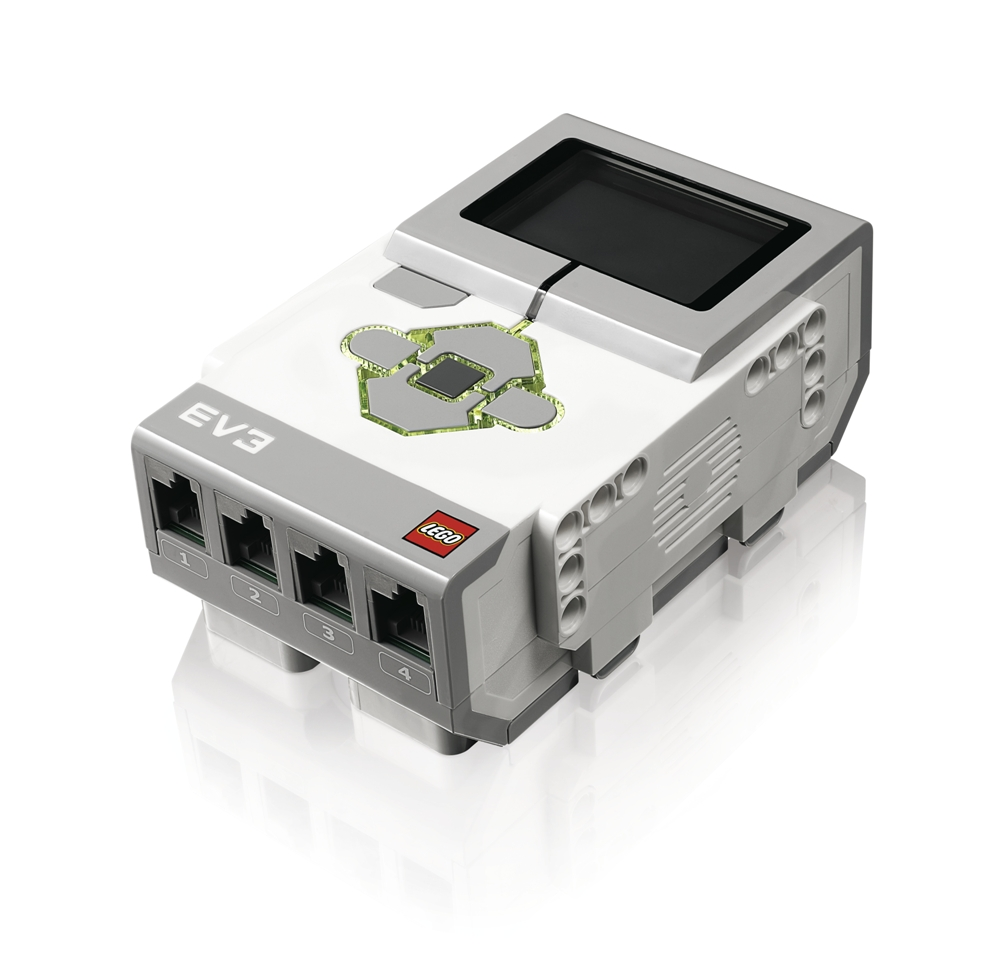
\includegraphics[width=330px]{images/lego-mindstorms-ev3_brick.jpg}
	\caption[\legoEV{ Brick}]{\legoEV{ \brick}\protect\footnotemark}
	\label{fig:lego-mindstorms-ev3_brick}
\end{figure}

\footnotetext{Zdroj: \url{http://hackeducation.com/2015/04/10/mindstorms}} 

Nová verze obsahuje také čtečku Micro SD karet, USB host interface a jeden výstupní port pro motory navíc (celkem 4~porty, NXT jen 3~porty) \cite{legoBotBench_comparing-EV3-and-NXT}. 

Slot na SD karty umožňuje rozšířit paměť pro programy, ale lze jej hlavně využít pro spouštění alternativních operačních systémů. 

Díky USB host interface lze k EV3 připojovat různé periferie, pro které je v systému a~vývojovém prostředí připravená obsluha.
% * <lucie.karmova@jcmm.cz> 2017-04-27T13:54:49.063Z:
% 
% > a
% Na konci řádku
% 
% ^ <paral.jarek@gmail.com> 2017-04-27T14:29:18.778Z:
%
% Opraveno.
%
% ^ <paral.jarek@gmail.com> 2017-04-27T14:29:20.221Z.
% * <lucie.karmova@jcmm.cz> 2017-04-27T13:54:32.207Z:
% 
% > nterfacu
% Neskoňujeme
% 
% ^ <paral.jarek@gmail.com> 2017-04-27T14:29:51.579Z:
% 
% Opraveno. Ok?
% 
% ^ <lucie.karmova@jcmm.cz> 2017-04-27T19:54:28.209Z:
%
% Sně.
%
% ^ <paral.jarek@gmail.com> 2017-04-27T20:24:42.349Z.
Lze tak připojit Wifi modul, klávesnici nebo myš. 
Zároveň můžete přes USB kabel spojit až čtyři EV3 \brick{\it y} a ovládat je jedním programem (z jednoho hlavního \brick{\it u}).

\begin{figure}[h]
	\centering
	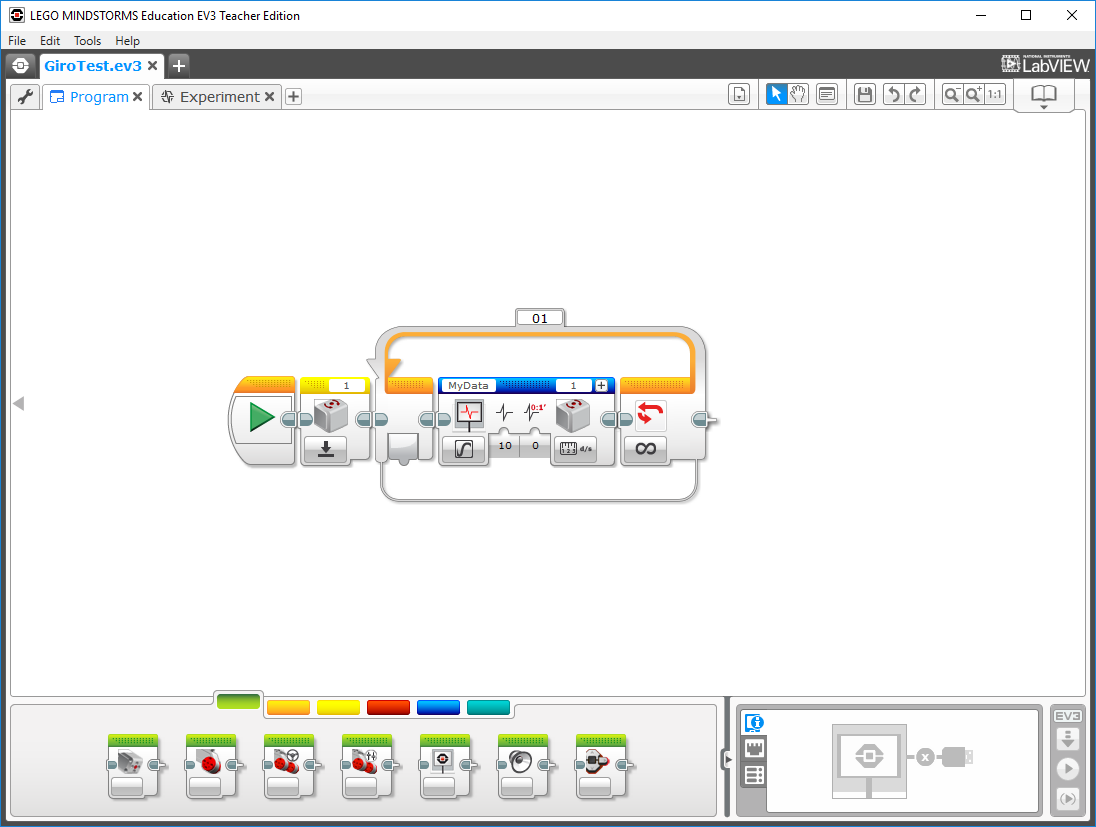
\includegraphics[width=\textwidth]{images/lego-mindstorms-ev3_dev-soft.png}
	\caption[\legoM{ }Education EV3 Software -- vývojové prostředí]{\legoM{ }Education EV3 Software -- vývojové prostředí}
	\label{fig:lego-mindstorms-ev3_dev-soft}
\end{figure}

Programovací prostředí pro EV3 je znovu postaveno na \labview{ }a ačkoliv se design v porovnání s prostředím pro NXT výrazně změnil (můžete porovnat obrázky \ref{fig:lego-mindstorms-nxt-g} a \ref{fig:lego-mindstorms-ev3_dev-soft}), neměli by mít uživatelé NXT s přechodem problém. 
% * <lucie.karmova@jcmm.cz> 2017-04-27T13:55:27.650Z:
% 
% > neměli by
% Před "neměli" chybí čárka
% 
% ^ <paral.jarek@gmail.com> 2017-04-27T14:30:46.323Z:
%
% Opraveno.
%
% ^ <paral.jarek@gmail.com> 2017-04-27T14:43:16.268Z.
Nové prostředí zvládne naprogramovat jak EV3, tak NXT \brick{}.
% * <lucie.karmova@jcmm.cz> 2017-04-27T13:55:53.147Z:
% 
% >  jak EV3, tak NX
% Párová spojka a máš správně čárky, pecka!
% 
% ^ <paral.jarek@gmail.com> 2017-04-27T14:43:43.939Z:
%
% To je pochvala? :-)
%
% ^ <lucie.karmova@jcmm.cz> 2017-04-27T19:54:40.382Z:
%
% Jo, fakt :-)
%
% ^ <paral.jarek@gmail.com> 2017-04-27T20:24:35.115Z.

V rámci alternativních platforem máme opět velký výběr \cite{legoMindstormsWikipedia_programming-languages}. 
Vhledem k nutnosti používání operačního systému je většinou pro dané prostředí potřeba nahrát konkrétní systém na SD kartu a spustit \brick{ }s touto kartou.

Jednotlivé alternativní platformy budou podrobněji probrány v následující kapitole.
